\begin{figure}[!ht]
\begin{center}

\begin{tikzpicture}
	\coordinate (A) at (0,0);
	\coordinate (B) at (1,-5);
	\coordinate (C) at (-3,-5);
	\coordinate (D) at (3,-3.5);

	\coordinate (UP) at (0,-4.25);
	\coordinate (DW) at (0,-10);

	\fill[brown](.3,-4.25)--(.3,-10)--(-.3,-10)--(-.3,-4.25);

	\fill[green](A)--(B)--(C);
	\fill[green!80!black](A)--(D)--(B);
\end{tikzpicture}
\end{center}
\end{figure}

\begin{figure}[!ht]
\begin{center}
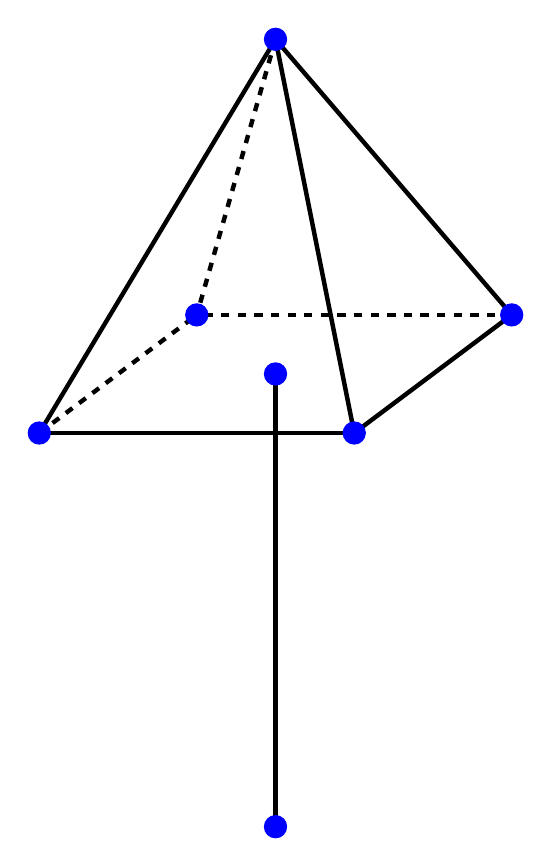
\begin{tikzpicture}
	\coordinate (A) at (0,0);
	\coordinate (B) at (1,-5);
	\coordinate (C) at (-3,-5);
	\coordinate (D) at (3,-3.5);
	\coordinate (E) at (-1,-3.5);

	\coordinate (UP) at (0,-4.25);
	\coordinate (DW) at (0,-10);

	\draw[ultra thick](UP)--(DW);

	\draw[ultra thick](A)--(B);
	\draw[ultra thick](A)--(C);
	\draw[ultra thick](C)--(B);
	\draw[ultra thick](A)--(D);
	\draw[ultra thick](B)--(D);
	\draw[ultra thick,dashed](A)--(E);
	\draw[ultra thick,dashed](C)--(E);
	\draw[ultra thick,dashed](D)--(E);


	\filldraw[blue](A) circle (4pt);
	\filldraw[blue](B) circle (4pt);
	\filldraw[blue](C) circle (4pt);
	\filldraw[blue](D) circle (4pt);
	\filldraw[blue](E) circle (4pt);

	\filldraw[blue](UP) circle (4pt);
	\filldraw[blue](DW) circle (4pt);
\end{tikzpicture}
\end{center}
\end{figure}

\begin{figure}[!ht]
\begin{center}
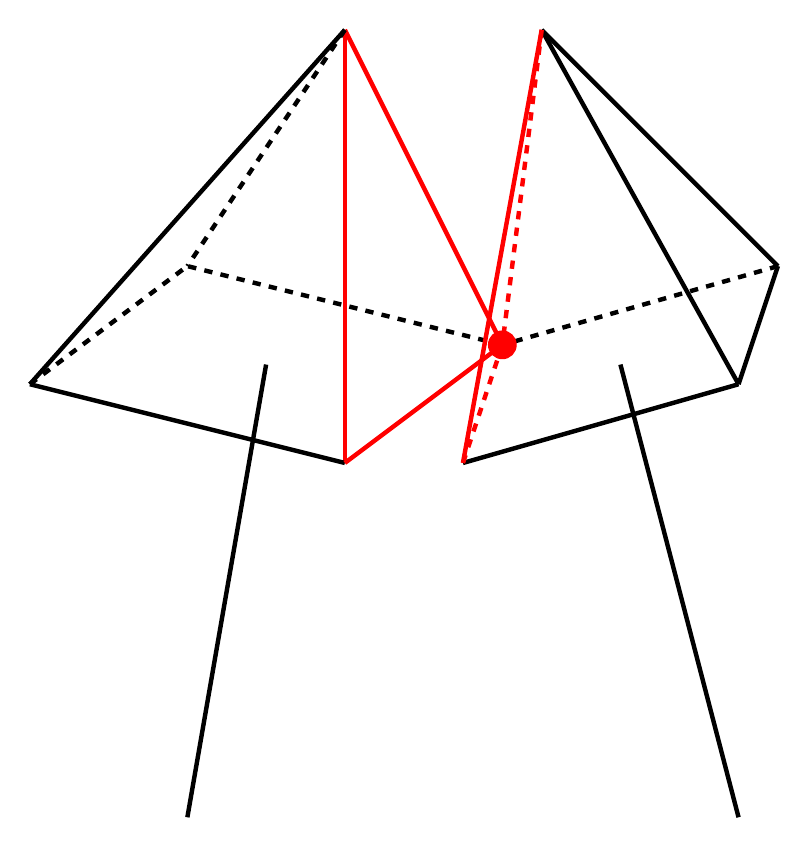
\begin{tikzpicture}
	\coordinate (A) at (1,0);
	\coordinate (B) at (1,-5.5);
	\coordinate (C) at (-3,-4.5);
	\coordinate (D) at (3,-4);
	\coordinate (E) at (-1,-3);

	\coordinate (UP) at (0,-4.25);
	\coordinate (DW) at (-1,-10);




	\coordinate (A2) at (3.5,0);
	\coordinate (B2) at (6,-4.5);
	\coordinate (C2) at (2.5,-5.5);
	\coordinate (D2) at (6.5,-3);
	\coordinate (E2) at (3,-4);

	\coordinate (UP2) at (4.5,-4.25);
	\coordinate (DW2) at (6,-10);




	\draw[ultra thick](UP)--(DW);

	\draw[ultra thick,red](A)--(B);
	\draw[ultra thick](A)--(C);
	\draw[ultra thick](C)--(B);
	\draw[ultra thick,red](A)--(D);
	\draw[ultra thick,red](B)--(D);
	\draw[ultra thick,dashed](A)--(E);
	\draw[ultra thick,dashed](C)--(E);
	\draw[ultra thick,dashed](D)--(E);

	\draw[ultra thick](UP2)--(DW2);

	\draw[ultra thick](A2)--(B2);
	\draw[ultra thick,red](A2)--(C2);
	\draw[ultra thick](C2)--(B2);
	\draw[ultra thick](A2)--(D2);
	\draw[ultra thick](B2)--(D2);
	\draw[ultra thick,dashed,red](A2)--(E2);
	\draw[ultra thick,dashed,red](C2)--(E2);
	\draw[ultra thick,dashed](D2)--(E2);


	\filldraw[red](D) circle (5pt);

\end{tikzpicture}
\end{center}
\end{figure}